\documentclass[11pt, oneside]{article}   	% use "amsart" instead of "article" for AMSLaTeX format
\usepackage{geometry}                		% See geometry.pdf to learn the layout options. There are lots.

\geometry{letterpaper}                   		% ... or a4paper or a5paper or ... 
%\geometry{landscape}                		% Activate for rotated page geometry
\usepackage[parfill]{parskip}    			% Activate to begin paragraphs with an empty line rather than an indent
\usepackage{graphicx}				% Use pdf, png, jpg, or eps§ with pdflatex; use eps in DVI mode
								% TeX will automatically convert eps --> pdf in pdflatex
\usepackage{amssymb}

\usepackage{hyperref} 				% you need this package
\usepackage{pifont}					% for \ding
\usepackage{url}					% I think needed for "plainurl" support in \bibliographystyle 

% Make clickable footnote
\newcommand{\hyperfootnote}[1][]{\def\ArgI{{#1}}\hyperfootnoteRelay}
  % relay to new command to make extra optional command possible
\newcommand\hyperfootnoteRelay[2][]{\href{#1#2}{\ArgI}\footnote{\href{#1#2}{#2}}}
  % the first optional argument is now in \ArgI, the second is in #1
  
% Takes at most 3 parameters (see http://www.tex.ac.uk/FAQ-twooptarg.html for info on multiple optional parameters)
% If first parameter isn't given, it's value is '' (empty string in text before footnote reference)
% If second parameter isn't given, it's value is '' (string before visible URL, e.g. 'http://')
% Makes a clickable footnote (alternatively: \url{}) with optional reference in the text as well
% Use 1: \hyperfootnote{www.mywebsite.com}: creates a footnote consisting of a clickable URL
% Use 2: \hyperfootnote[My website]{www.mywebsite.com}: creates a clickable piece of text in the text ('My website') plus a footnote consisting of a clickable URL
% Note: requires the hyperref package.
% Note: use xspace package to add/absorb spaces when necessary (e.g. to avoid a space between the footnote number and a punctuation mark)

% Info on how to define a LaTeX command: https://www.sharelatex.com/learn/Commands

%SetFonts

\title{Identity Agents}
\author{Paul Trevithick, The Mee Foundation}
\date{Created March 3, 2023. Revised: \today}							% Activate to display a given date or no date

\begin{document}

\maketitle
\begin{abstract}
There is a power imbalance between digital service providers and their users, with regard to these users' personal information and online identity. Users lack of autonomy and agency, are subjected to third-party surveillance, and are inconvenienced by a provider-controlled, siloed architecture that manages their personal information. We explore design considerations for potential solutions and propose a design for an \emph{identity agent} and associated legal contract, that represents the user and protects their interests online.
\end{abstract}

\section{Power imbalance}
While the internet has brought new services and experience to billions of users, it has also resulted in a power asymmetry between the digital service providers and their users regarding these users' digital identities and personal data. 

The internet's designers, in the interest of resilience and scalability began with a decentralized architecture that pushed computation and storage to the edge and minimized centralized control. However, in recent decades economic factors, so-called natural monopolies, preferential attachment network effects, economies of scale, and the relative ease of creating centralized solutions have all contributed to concentrations of power into the hands of a few relatively large providers providing services to billions of users. 

Berners-Lee invented the web as a decentralized platform wherein anyone could publish a website and link to any other site. He even envisioned that these pages would be editable. However, as the web has grown from a research-sharing community into a global medium for commerce, communication, journalism and entertainment, power has concentrated. Today, the web is dominated by enormous companies like Amazon, Meta, Google, and Netflix. These corporate giants enjoy enormous control not only over what people see and do online, but over their users' private data.\cite{Finley2017}

In response, many initiatives have arisen proposing alternative approaches and technologies. Here are just a few representative examples: \hyperfootnote[rececentralize.org][https://]{redecentralize.org}, \hyperfootnote[DWeb principles][https://]{getdweb.net/principles/}, \hyperfootnote[The Web3 Foundation][https://]{web3.foundation/}, \hyperfootnote[the Decentralized Identity Foundation(DIF)][https://]{identity.foundation}, \hyperfootnote[``local-first" software principles][https://]{inkandswitch.com/local-first/}, \hyperfootnote[ProjectVRM][https://]{blogs.harvard.edu/vrm}, \hyperfootnote[Blue Sky][https://]{blueskyweb.xyz/}, and Berners-Lee's \hyperfootnote[Decentralized Information Group][https://]{dig.csail.mit.edu}. 

We use the term \emph{user agent} to refer to software tools that work (i.e. provide agency) ``on the user's side" for, and \emph{exclusively} on behalf of, the user. Since our discussion applies equally to provider's mobile apps, webapps, and websites, from here forward we will simply use the term \emph{app} to refer to all of them.

Power asymmetry lies at the root of a diverse set of related end-user symptoms, most of which erode privacy, since privacy and power are highly interrelated concepts\footnote{Consider the title of V\'eliz's recent book, ``Privacy is Power"\cite{veliz2020}}. 
These privacy-eroding symptoms include a lack of personal autonomy, a lack of personal agency, and third-party surveillance. 

\subsection{Lack of Autonomy}

\begin{quote}
\textbf{au\hspace{0.5mm}\tiny \ding{108}\normalsize \hspace{0.5mm}ton\hspace{0.5mm}\tiny \ding{108}\normalsize \hspace{0.5mm}o\hspace{0.5mm}\tiny \ding{108}\normalsize \hspace{0.5mm}my}: \emph{freedom from external control or influence; independence.}\hyperfootnote[][https://]{languages.oup.com/google-dictionary-en/}
\end{quote}

\emph{Independence}. In real life each of us is an independent entity. Each of us has a self that embodies our individuality. We ``bring" that independent selfness to interactions with others, with vendors, etc. while understanding that this independence is not absolute--we are still to some extent dependent on common, shared systems, laws, environments, and so on. By contrast, it has been said that ``we have no \emph{digital embodiment}."\footnote{Phil Windley, personal communication, Sepember 2022}  Our identities are provided to us by digital service providers (e.g. in the form of a Facebook identity, or an Amazon account). Without them we don't exist. Anyone who has been banned from a platform, or uses a platform that has been shut down is sharply reminded that their digital identity exists at the pleasure of that platform. Our provisional existence is the original power asymmetry. Efforts create personal datastores, or more specifically, those that strive to provide each of us a \emph{self-sovereign identity}\cite{Preukschat2021} are squarely aimed at addressing this issue--the word ``sovereignty" certainly evokes power. Lanier refers to this as a person's right to a ``First-class identity."\cite[p251]{Lanier2014}.

\emph{Ownership}. Our personal data is collected and held by organizations as we interact with their apps, but not by us. This pattern \emph{app-held data} by \emph{first-parties} is so common that it's hard to imagine an alternative. Our data is not free from external control by apps, because it is generally stored and managed by them. Our data is also collected and held by \emph(third-parties) (e.g. data brokers) with whom we have no direct interactions. In short, it's been said that \hyperfootnote[“everybody has our data … except us.”][https://]{reb00ted.org/personaldata/20210620-who-has-my-personal-data/}. 

As we'll discuss more later on, there alternatives have been proposed. One is ``user-held" data\cite{Jurcys2021}, where your data is held by you in a personal datastore\footnote{Examples of open-source personal datastores include \url{https://solidproject.org}, Decentralized Web Nodes(DWN). For more about personal datastores see \url{https://wikipedia.org/wiki/Personal\_data\_service}}. Another is following ``local-first" software principles.\cite{Kleppmann2019}

\emph{Lock-in}. As we've mentioned our online existence is provisional. Our existence is bound to the provider from which it originated. Providers hold our data, and although in many jurisdictions providers are required to allow us to have access (e.g. to request that we can download a copy), we lack the technical means to accept the data stream and store it under our control (e.g. in a personal datastore). If we did we'd have the potential to subsequently transform it into other formats and thereby make it reusable in other contexts. Thus our data is held hostage, i.e. without autonomy. 

\emph{Peer-to-peer} With a few exceptions\hyperfootnote[][https://]{berty.tech}, internet users, when they communicate person-to-person don't have the ability to do so \emph{peer-to-peer}--from their edge device to the other person's device. Instead, they are dependent on servers hosted by intermediaries. Whereas it is now standard practice that the content of messages is end-to-end encrypted, the metadata about them (e.g. who a person communicates with, from where, at what time, how often and from which device, etc.) is in many cases visible to the intermediary server. 

\subsection{Lack of agency}

\begin{quote}
\textbf{a\hspace{0.5mm}\tiny \ding{108}\normalsize \hspace{0.5mm}gen \tiny \ding{108} \normalsize cy}: \emph{the capacity, condition, or state of acting or of exerting power} \hyperfootnote[][https://]{www.merriam-webster.com/dictionary/agency}
\end{quote}

\emph{Wielding credentials}. In real life you can present your drivers license to a wine seller in order to prove that you are of drinking age since the wine seller trusts the license issuer. The interaction is privacy-respecting because the presentation interaction is not disclosed to the issuer. This could be described as \emph{wielding} a trust credential. At present, there is no equivalent way to do this online. There's no standard way to be issued a credential, hold it in digital wallet, and then present it. With a few, domain-specific exceptions (e.g. cryptocurrency), there is no standard online method for you to prove something one party states about you, to another party.

\emph{Data presentation}. One reason providers' apps rely on form filling and other kinds of data entry is that the user, even one equipped with a personal datastore, lacks the ability to present personal information digitally to the provider. Instead, the information must be re-entered manually at each provider. The credential presentation interaction mentioned is another example of this.

\emph{Delegation}. In the offline world one entity can grant access to some resource to another entity. For example, I can give my car keys to a friend so they can borrow my car. There is no standard, secure way to do this online. This is especially problematic in healthcare scenarios where a healthcare provider needs access to electronic health-related data about a patient, whereas the patient may not be able to provide it by themselves but instead needs to rely on someone else, e.g. a family member to grant the needed permission.

\emph{Provider-defined Privacy Policies}. As is expected, providers define policies which are designed to protect the their interests while staying within the limits defined by the relevant privacy regulations. Users are indeed given the option to review these policies with the burden of making sense of them shifted to the user (i.e. the potential victim). Because the user typically uses dozens providers or more, they don't have the time to review each of these policies and they lack user agents to assist them. 

\emph{Privacy policy expression}. With a few exceptions, (e.g. the \hyperfootnote[Global Privacy Control][https://]{globalprivacycontrol.org}), users  lack the technical means (i.e. computational capability) to express their own privacy terms to providers. 

\emph{User rights}. In a growing number of jurisdictions, including Europe under \hyperfootnote[GDPR][https://]{gdpr-info.eu/} and California under \hyperfootnote[CPRA][https://]{thecpra.org/}, the user's data rights, (e.g. the right to access, correct and delete their data), are clearly described. In principle these laws respect these rights, however in practice the time and effort required to exercise these rights at every app/site is sufficiently onerous, that in practice they are not respected. The user must send written requests to get copies of their data, update it, or have it be deleted. The power of user agents is necessary to regain in practice, the rights they already have in principle. 

\emph{Content filtering}. Social networking platforms have replaced human content editors with algorithmic filters. Users might think that they see a balance of content whereas in reality they are trapped in what Pariser called ``filter bubbles."\cite{Pariser2011} Pariser's recommendation is that if platforms are going to be gatekeepers, they need to program a sense of civic responsibility into their algorithms, they need to be transparent about the rules that determine what gets through the filter, and ``they need to give user control of their bubble."\cite[p66]{McNamee2020}

\emph{Behavioral advertising}. Behavioral, (aka targeted) advertising involves the automatic generation of interest profiles by third-party adtech firms. In most cases users have no control over these interest profiles, and no ability to correct them.

\subsection{Third-party surveillance}

Whereas the user is at least aware when they sign up on a first-party app that their interactions are known to the provider of that app, there are also hundreds of third-parties of which the user is unaware that track and assemble databases about them. Databases of user data in the hands of hundreds of unknown third-parties creates privacy risks and vulnerabilities. Users have no visibility into what's being gathered, where it's being shared, and how it's being used. It is worth noting that that much of this third-party tracking is enabled in collaboration with first-parties (e.g. first-parties placing third-party tracking cookies on the user's browser).

\emph{Surveillance-based targeted advertising}. Targeted advertising \footnote{Also known as behavioral advertising, or more recently, interest-based advertising} involves four main processing steps: (i) the collection of observations about the user by a first- or third-party, (ii) synthesis of an "ad profile” from these observations, (iii) matching this ad profile against available "target audiences”(i.e. characteristics of whom the advertiser wishes to reach, advertising budget, etc.) from advertisers through a bidding process, and (iv) displaying the winning ad. Surveillance-based targeted advertising specifically is when step (i) above is achieved by third-parties who track the user as they move from apps to app and site to site across the internet using third-party cookies and other tracking mechanisms. 

\emph{Data brokers}. Data brokers are third-parties who buy and sell personal data to other brokers, to advertisers, adtech firms and first-party publishers. They provide  personal data marketplaces and exchange behind the users's back, because users lack user agents to provide data about themselves.


\subsection{Inconvenience}
The prevailing architecture of the internet involves each provider managing their own  information ``silo" of information about the user (i.e. their account). This approach and the lack of sufficiently powerful user agents creates inconvenience.

\emph{Repetition}. When using apps, users are often asked to provide information about themselves that another app has already asked them, such as ``what is your email address?" This is a symptom of the internet's silo-ed architecture wherein each app maintains its own database of personal information. The user has the hassle of repeated data entry and the app offers a less-than-optimal user experience.

\emph{Password management}. The average user uses 100 websites and 25 apps daily. Although managing and periodically updating strong, unique passwords at each is  impractical without an automated password manager user agent, it has been estimated that less than five percent of internet users use one. 

\emph{Account Management}. The user shoulders the burden of maintaining the timeliness and consistency of their account information at dozens of apps. For example, updating contact or credit card information at each is tedious, time-consuming and encourages the user to spend more time at sites that already have their information. The relative convenience of shopping on Amazon vs. another e-commerce site is a consequence partially caused by the user's lack of a user agent to manage these relationships.


\section{Design Considerations}%Design Considerations

In this section, we discuss a number of design considerations for any solution to successfully address the symptoms just described.

\subsection{User-centric vs. provider-centric}

Many of the challenges described thus far have their origin in an architecture that is \emph{provider-centric} rather than \emph{user-centric}, or \emph{human-centered}. The internet is comprised of millions of providers, each offering their own app[s]. In this provider-centric model the user is viewed insolation--the fact the that user uses apps from dozens of providers is irrelevant from any given providers's perspective. Each provider's app sees a single narrow slice of the individual through the lens of their direct interactions with them. Each works in isolation to optimize the user's experience on their app or at their site. 

To the individual the situation is reversed. They use many dozens of apps with connections to each app radiating out from them. The individual at the center has the burden for entering, and updating personal information, payment details, preferences, and so on at each.

User-centric technologies that are designed to empower the user across multiple apps from multiple providers are called are \emph{user-agents}. A web browsers is an example, especially it's built-in form-filler which reduces the number of manual keystrokes required to fill in web forms. Another example is a password manager. 

\subsection{Edge-centered vs. cloud-centered}
Assuming that user-centric decentralized architecture is required, a related question is where should the user's agent and associated personal datastore live? Should it be edge-centered, or cloud-centered? Edge-centered means that the primary location for a user's agent is on their own phones, and laptops and perhaps home servers. Cloud-centered means that the user's agent is primarily held in the cloud (e.g. on a \hyperfootnote[SOLID][https://]{solidproject.org} pod). We say \emph{primary} because there are usually use-cases that involved replicating/syncing some of the data to the ``other" location. Both options have their advantages and disadvantages, we explore three of them here.

\emph{Security}. Although this is debatable, it is our contention that having a personal datastore on a personal, edge device is more secure than in the cloud if we assume a large number of users. Even if each  alternative were equivalently secure for a single user, a cloud-centered architecture inherently aggregates large numbers of personal datastores at one cloud service provider and thereby creates a much larger economic incentive for hackers to invest in attacking it. 

\emph{Equity}. The hosting costs of a cloud-centered solution must be paid for by someone, whereas user's typically own their edge devices and they are thus on a marginal basis for a new app essentially ``free". Solutions must be able to be afforded by all socio-economic classes and not just those better off. On this basis we believe solutions that incur monthly hosting fees are disqualified.

\subsection{Replication}

If we assume an edge-centered design, we introduce the need to solve the related, so-called \emph{roaming} problem. That is, we must support use cases wherein the user has more than one device that are intermittently connected to the internet, and needs to have their personal datastore state be consistent across these devices, at least eventually. This requires that the user's agents implement data replication and syncing between themselves. An open research question is how to achieve this replication without the need for relay servers and their attendant costs--costs which undermine the equity consideration previously mentioned.

\emph{Backup}. One disadvantage of so-called \emph{non-custodial}, edge-centered architecture (as compared to cloud-centered architectures) is the vulnerability of users who are not diligent about backing up their devices (e.g. to an online service) to losing their agent-managed personal data. For users with more than one device this is less likely since data is replicated (as mentioned above) across their devices and a repaired or replaced device's data can be restored from one of the user's other devices. There remains of course the worst-case scenario wherein the user didn't backup any of their devices and all of them at the same moment are lost or damaged. 

\subsection{Loyalty}

Much of the power asymmetry described in the first section is due to economic incentives for providers to motivate them do just enough in the user's interest to keep them as a user or customer, but not more. Personal data, after all, is considered by business to be an asset class and thus the more of it that is collected and monetized the better. If an agent is to work \emph{exclusively} on behalf of the user, the agent provider must not have an economic incentive to provide anything less than complete loyalty to the user's interests. 

Although there are other potential solutions (e.g. data cooperatives and data unions) one of the simplest is that the agent provider be a nonprofit organization that has no economic interest in the user's data. This being the case, there is no need for the agent provider to have any access to the user's data.

\subsection{Metacontextual}

Zuckerberg once said ``Having two identities for yourself is an example of a lack of integrity"\cite{Kirkpatrick2011}, but even if you can force all users of a single system like Facebook to have a single identity, this approach is unworkable for the design of an agent that represents the user across multiple, widely varying systems and contexts. People need the freedom to be themselves--selves that are complicated and messy. Our identities vary depending on whom we are interacting. We choose to express different parts of ourselves within different contexts. Not only are the attributes we share different the values of one attribute may be different in different contexts. 

\begin{quote} ``[A]t various times in the same day, virtually every adult can be a friend, a worker, a supervisor, a citizen, a mentor, a student, a musician, a customer, a lover, a child and a parent. Each of these roles demands different behavior and different aspects of our selves, aspects that need not be consistent. We behave, for example, in different ways with loved ones than with those we encounter in commercial or professional settings. Even among our loved ones, we behave very differently (and often show very different sides of ourselves) to our children, our parents, and our sexual partners. But this is not dishonest, nor is it inconsistent. At the very least, it's no more inconsistent than is the complicated nature of having a self. It is human."\cite[p122]{Richards2021}
\end{quote}

If we look at a person's age attribute we see that across several contexts they might share, respectively, their exact chronological age among one's close friends, a fictional age to a music recommendation service, no age at all in contexts wherein doing so might cause discrimination against them, or a merely a statement that they exceed the legal drinking age. 

In his \hyperfootnote[last public speech][https://]{www.youtube.com/watch?v=9DExNTY3QAk}  
\hyperfootnote[Kim Cameron][https://]{en.wikipedia.org/wiki/Kim\_Cameron\_(computer\_scientist)} introduced two useful definitions based on archaic English:

\begin{itemize}
\item \textbf{Selfness}: The sameness of a person or thing at all times or in all circumstances. The condition of being a single individual. The fact that a person or thing is itself and not something else. Individuality, personality. 
\item \textbf{Whoness}: Who or what a person or thing is. A distinct impression of a single person or thing presented to or perceived by others. A set of characteristics or a description that distinguishes a person or thing from others. 
\end{itemize}

The following diagram illustrates these concepts and introduces the notion of context:

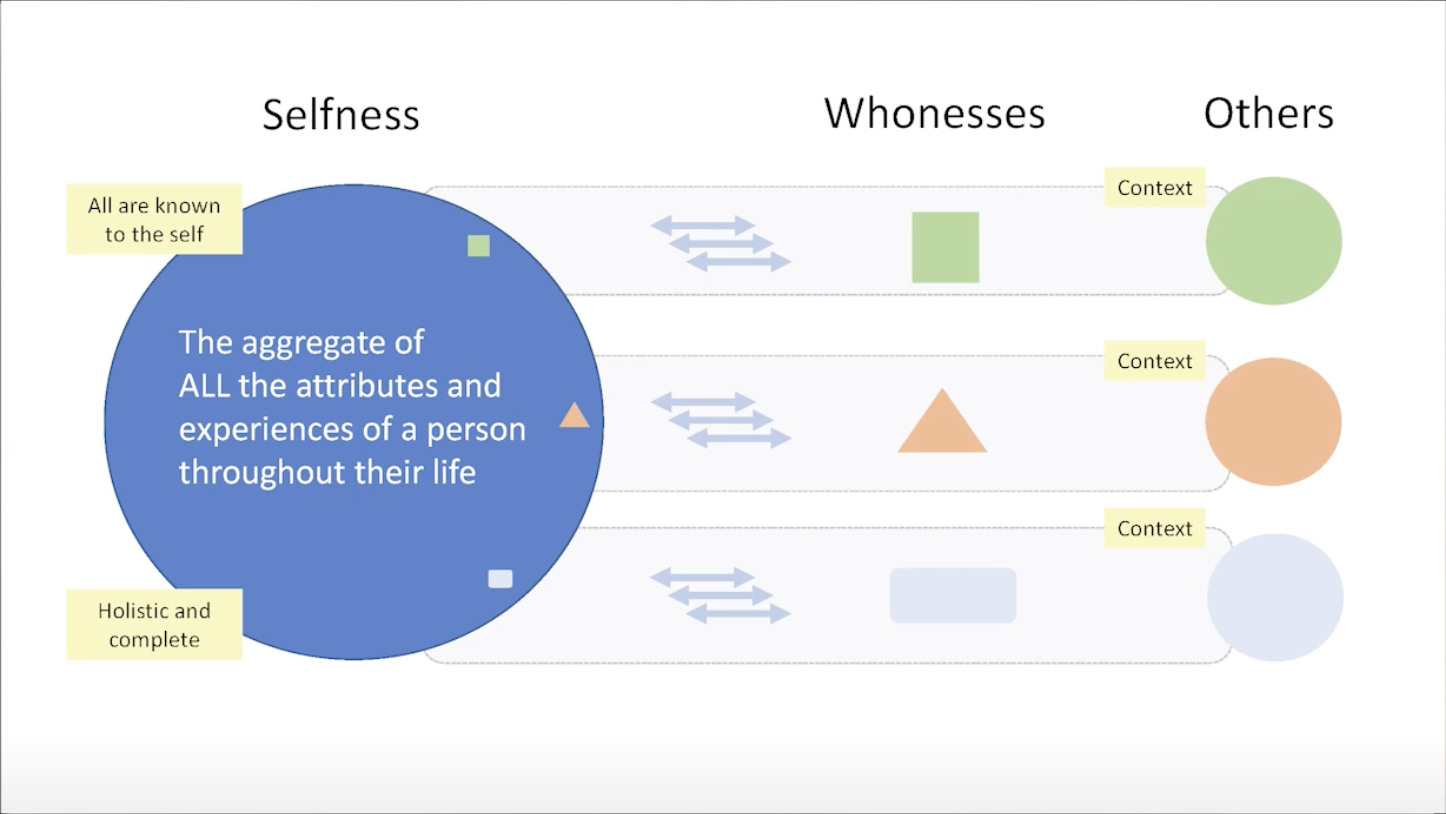
\includegraphics[width=\textwidth]{./images/selfness-and-whoness-larger.png}

Using these terms we can say that in everyday life people have one \emph{selfness}, but they have many, context-dependent \emph{whonesses}. 

\subsection{Delegation}

In \emph{A Human Rights Approach to Personal Information Technology}\cite{Gropper2022} Gropper asserts that there is an architectural principle that must be adhered to in order to respect human rights [e.g. to privacy]. He itemizes three universal components of the personal information commons:

\begin{itemize}
\item \textbf{Authentication} (signing-in and signing documents)
\item \textbf{Request} for information (e.g. forms, searches, conversations)
\item \textbf{Storage} (e.g. labs, prescriptions, social contracts, transactions [, other human information])
\end{itemize}

What could be called the \emph{Gropper Principle} is this (our words, his ideas):
\begin{quote}
``Any system that respects the human right to privacy must not bundle authentication, request, and storage."
\end{quote}

In his presentation\hyperfootnote[][https://]{identiverse.com/idv2022/session/841489/} at the 2022 Identiverse conference provides additional detail (see \hyperfootnote[slides][https://]{drive.google.com/file/d/1lwaMVkG4kLi7z6cXhqMx-DGkUww9azW3/view}). It explains that only a decentralized architecture can implement the Gropper Principle because each of the three concerns needs to be implemented separately. For this to work in an open world with multiple alternative component providers, we as a development community will need to converge on open standards between and among these three components. 

\subsection{Trustworthiness}

Any agent solution for online identity is by it's nature managing highly sensitive information. In order to be adopted voluntarily by people any solution must be trustworthy--its users must have confidence that their information isn't being used against their interests. 

Solutions based on open source software can leverage transparency to help build this confidence that the solution is trustworthy. In open source software the source code is visible to anyone to review and audit to ensure that the solution is secure, free from vulnerabilities, and works in the user's interest.

In addition to open source, users will also consider the nature of the organization offering the solution as to trustworthiness. The organization's financial incentives should be aligned with their users interests. In this regard a nonprofit organization can be created that has no financial or business incentive to exploit the user's data against the user's interest. Ideally the organization would have no need to have any access to the user's data so that there's simply no reason to have to trust them, their security infrastructure and practices.

\subsection{Data Governance}

Once data is shared from the agent to a first-party there are no technical means to constraint what the recipient does with it. No technical means can prevent them from selling it others, for example. Instead, legal means must be employed. Rather than wait for privacy regulations to get strong enough, we propose that first-parties sign a Human Information License to license the user's information under terms that are fair and balanced and respect the user's privacy rights. This contract can be signed by an entity that represents the user and makes it effortless for them.

\subsection{User rights}

People should enjoy user rights to access, correct and delete their own personal information managed by providers. Unfortunately, even the best privacy legislation while providing these rights in principle, does not do so in practice. The reason they fail in practice is that the combined burden of the mechanisms to exercise these rights across dozens of apps, is unmanageable for the user. To provide these rights in practice, providers must implement APIs and user's must have user agents that can consume them on the user's behalf.

\subsection{Enforcement}

[to-be-written: Talk here about the need for an entity to audit and enforce compliance with the legal contract]

\section{Identity Agents} 

\subsection{End-user perspective}
An \emph{identity agent} is an app that gives the user control (power) over their own personal information as they interact with websites, mobile apps, and other user's agents. It does this through a combination of technical and legal mechanisms.

\subsubsection{Privacy and Autonomy} 
The agent runs on the user's edge devices (mobile phone, laptop, etc.) where, entirely under the user's control, it holds a local, private database of the user's personal information. When an app/site wants to know something about the user, the agent shares as much or as little as the user chooses. If an app/site signs a Human Information License and thereby becomes \emph{certified}, the legal entity behind that app/site is thereby obligated to (i) require explicit consent for collection, processing, storage and sharing of the users data and to (ii) implement APIs to exercise the user's rights to access, correct and delete the user's personal information. We envision that agents could provide ad profiles to certified publisher websites that are supported by interest-based advertising while eliminating the need for surveillance by third-parties.

\subsubsection{Convenience}
Although the agent is an interactive application, it operates in the background most of the time. Always working solely in the user's interest, it collects information from sites that already hold their data, and shares it with other sites that need it. Our vision is that that the user \emph{never has to repeat themself} (nor remember passwords!) as they move from app to app and site to site across the internet.

Here are a few examples. If a site wanted to know the user's email address it might ask for it in a web form. In this case the agent would use it's form-filler ``protocol" to fill in the value. If the site supports password-less sign-in (e.g. using OpenID Connect) the agent acts as the identity provider. If a site needed a digital driver's license credential, the agent acts as a digital wallet and presents this credential that it had presumably downloaded earlier from an issuing site. In these different examples, different protocols for information sharing would be used, and the agent must be technology agnostic and support all of them. Only in this way an an agent be human-centric and put the one user at the center of all of their online relationships.

\subsection{Self and contexts}
The agent represents both the user's single \emph{selfness} and their multiple context-dependent \emph{whonesses}.

The selfness of the user is held in a data container called the \emph{self}. The contents of the self are holistic and therefore quite sensitive. For this reason they would normally not be shared in a direct or comprehensive form with others. The user's self is the point of integration across contexts each of which may be from differing identity systems, use different protocols for communication and different schemas for knowledge representation.

Each context is represented by a \emph{context} data container. A directed \emph{correlation} link points from an entity in the self to the entities representing the user in each context. To ensure privacy only the user knows that each of these separate contexts contain representations of them. Each context represents an interaction via some communications protocol with an external app, website or agent. 

We can illustrate these concepts with a simple example. A user might play a game on a gaming site using the id DevilSpawn666, while communicating on Twitter as @alicewalker and subscribing to the New York Times as alice.walker@gmail.com. Here's a simplified view of how this is represented:


\includegraphics[width=\textwidth]{./images/example1.png}

\subsection{Functionality}

Here is a summary of the functionality of an example agent.

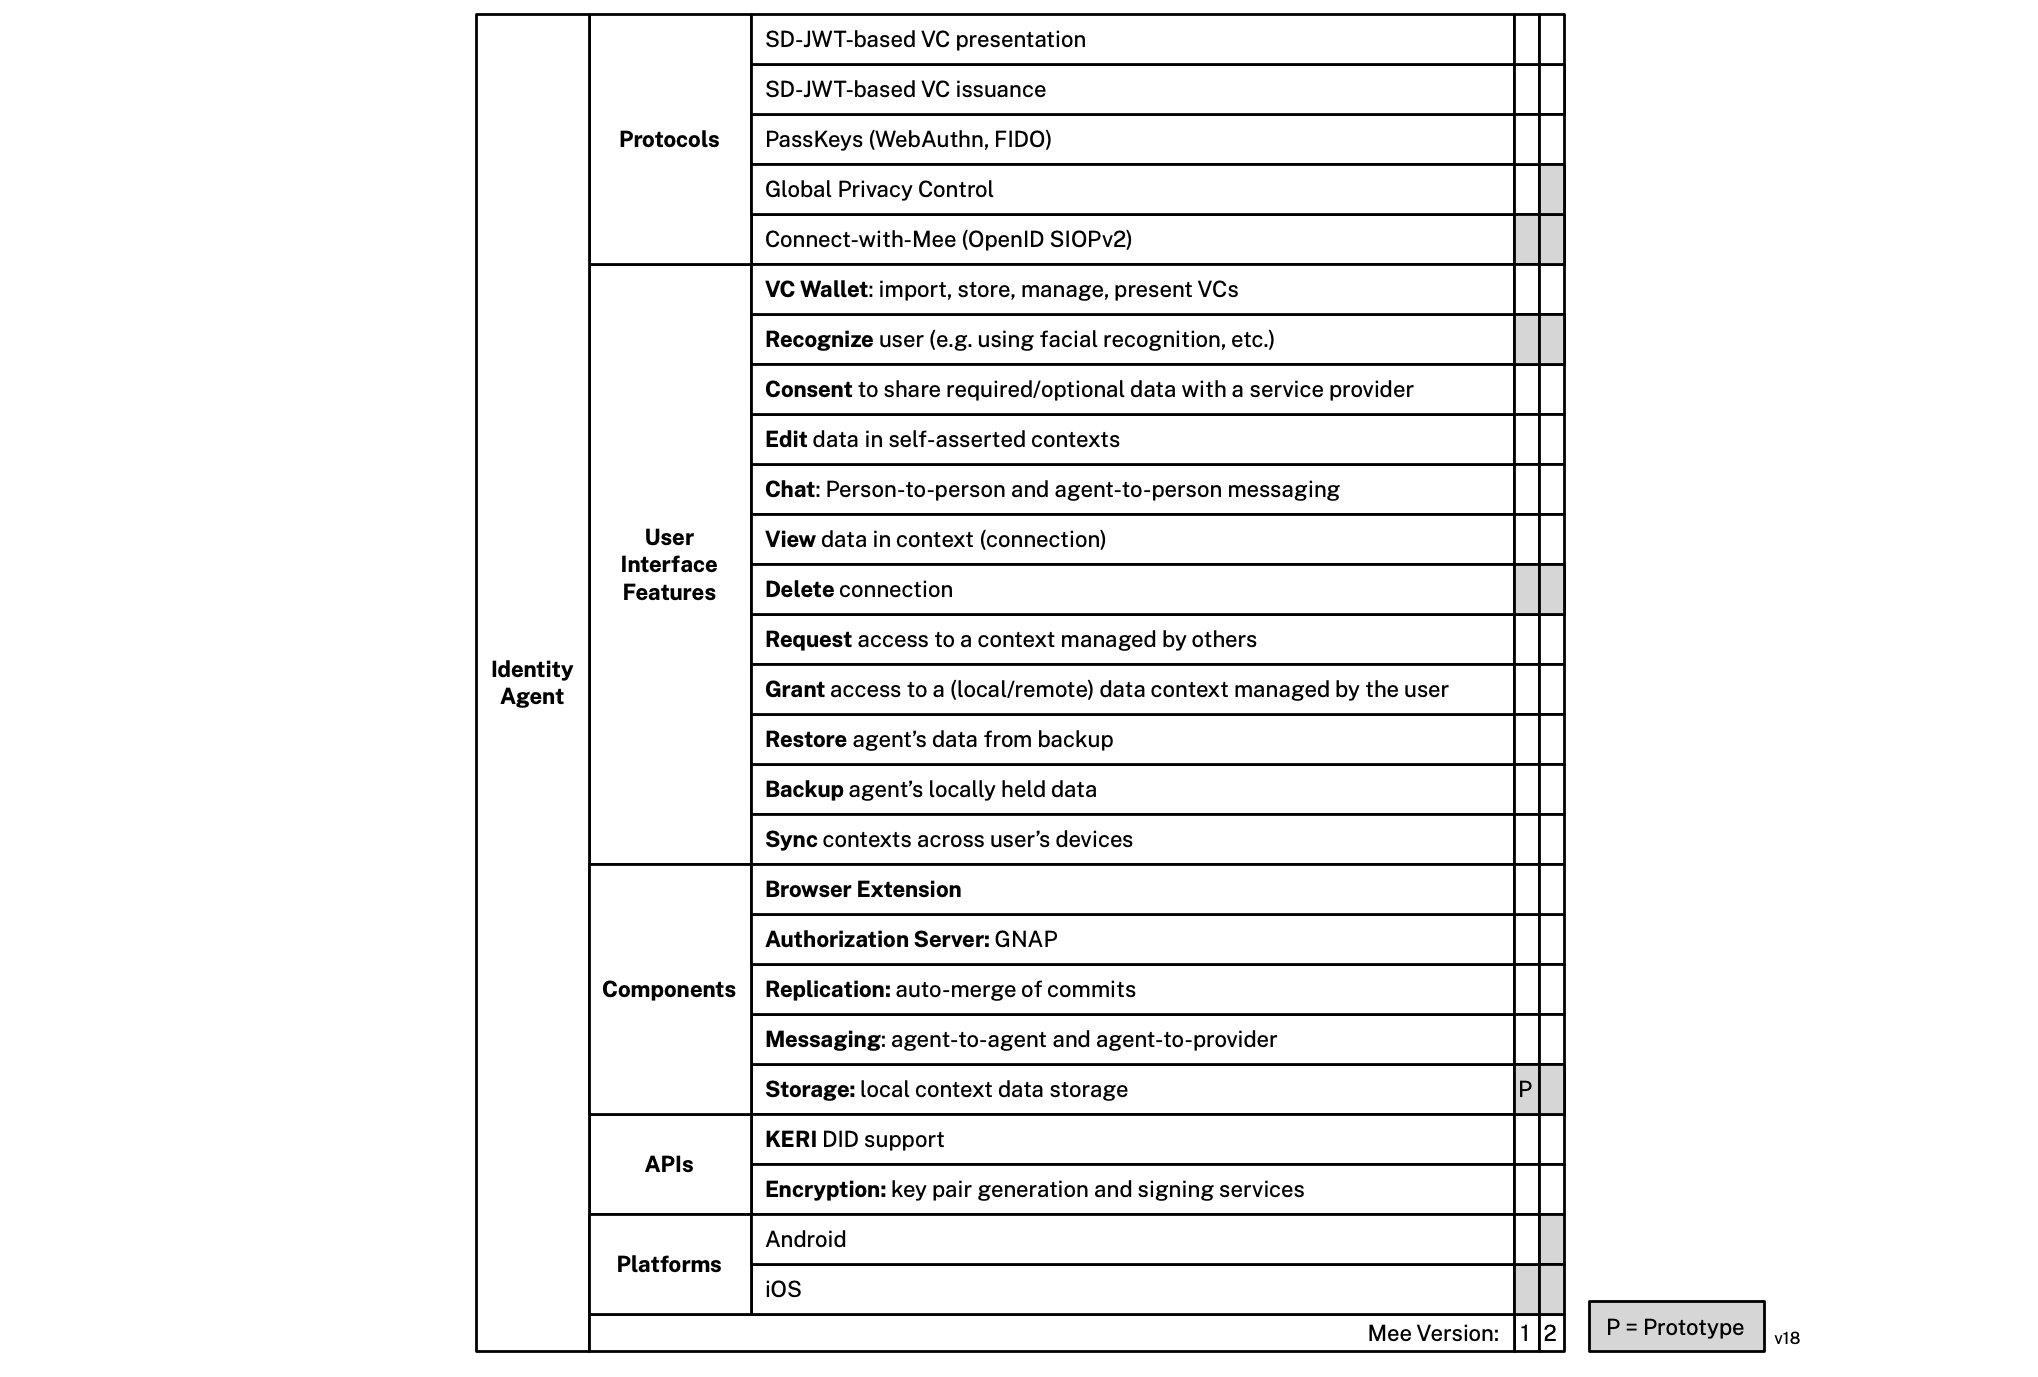
\includegraphics[width=\textwidth]{./images/agent-functionality.png}

\subsubsection{Protocols}

\begin{itemize}
\item SD JWT-based VC presentation
\item SD JWT-based VC issuance
\item PassKeys (WebAuthn)
\item Global Privacy Control
\item Connect-with-Mee: (OpenID SIOP) that uses a universal link to the agent
\end{itemize}

\subsubsection{UI Features}

\begin{itemize}
\item \textbf{VC Wallet:} import, store, manage, and present Verifiable Credentials (VCs). Note: the [OWF conceptual architecture](https://github.com/openwallet-foundation/architecture-task-force/blob/main/docs/architecture/conceptual-architecture.md) adds Burn, Receive, Send, Transfer, Refund, Purchase, Withdrawal, Deposit
\item \textbf{Recognize} user (e.g. using facial recognition, etc.)
\item \textbf{Consent} to share required/optional data with a service provider
\item \textbf{Edit} data in self-asserted contexts
\item \textbf{Chat:} Person-to-person and agent-to-person messaging
\item \textbf{View} data in contexts
\item \textbf{Delete connection} delete all data associated with this set of contexts
\item \textbf{Request} access to a context managed by others
\item \textbf{Grant} access to a (local or remote) data context managed by the user
\item  \textbf{Restore:} recover all data using SRP and backups
\item \textbf{Backup} local contexts
\item \textbf{Sync} contexts across user's devices
\end{itemize}

\subsubsection{Components}

\begin{itemize}
\item \textbf{Authorization Server}: GNAP AS
\item \textbf{Replication}: synchronization of context state across the user's set of agents
\item \textbf{Messaging}: communications among members of the user's set of agents
\item \textbf{Storage}: local data storage for contexts  
\end{itemize}

\subsection{Architecture}

In this section we propose an architecture for identity agents. We consider a user, Alice, and her agent's three layered architecture shown below.

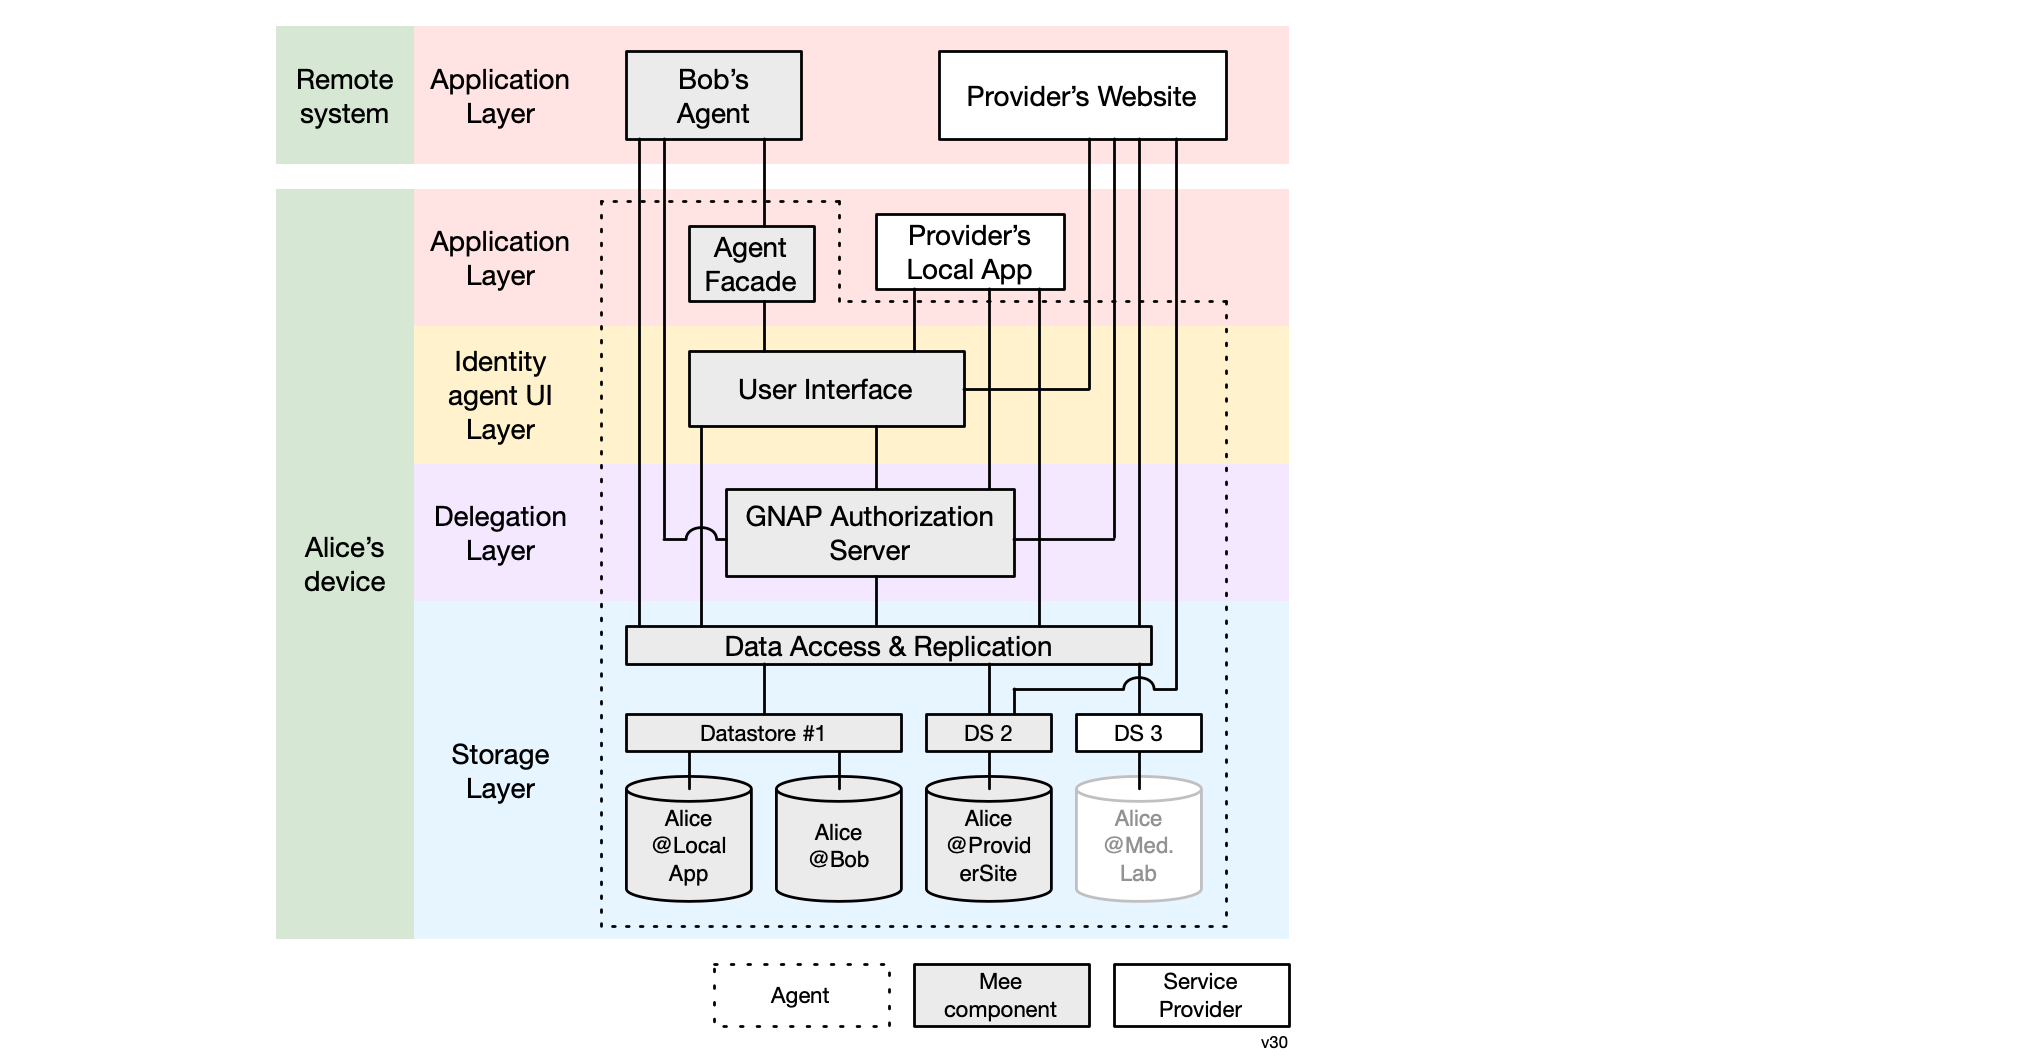
\includegraphics[width=\textwidth]{./images/architecture.png}

\subsubsection{UI layer}

Alice's identity agent is deployed as an app on Alice's device (e.g. a smart phone). The top, UI layer provides Alice with data management features to connect with apps/sites and manage her data. This UI allows her to inspect and in some cases edit each of the partial representations of her in each connection's context(s). Part of this UI is an "agent facade"--a presentation layer for how Alice appears to other agent users. 

\subsubsection{Delegation layer}

The \hyperfootnote[GNAP][https://]{oauth.net/gnap/} Authorization Server (AS) responds to requests for access to Alice's context datastores wherever they may be located physically. These requests could come from any app/site whether local or remote. In other words they could come from local apps (e.g. Provider's App), remote app/sites (e.g. Provider's Website) or from other users' agents (e.g. Bob's Agent). The AS is integrated with the agent's UI to allow Alice to grant or deny these requests for access. If Alice, either through explicit UI interaction or via a policy she has established, grants the request, the AS returns an access token to the requester. The requester presents this access token to a context datastore when it needs access. 

\subsubsection{Storage layer}

The Data Access and Replication component has two responsibilities. First, it provides an abstraction layer performing schema mapping such that the UI layer with which it is integrated has read/write access to context data in an abstract, universal schema. This is the ``data access" responsibility. The second responsibility is to manage the replication of data within Alice's context datastores across all of Alice's devices (phone, tablet, laptop, etc.). 

Below the Data Access and Replication component lie a set of datastores each using its own datastorage technology to hold one or more contexts (data containers). Each context holds a contextualized representation of Alice as defined (as to schema) and created and managed by apps/sites. The diagram above shows three local contexts on Alice's device and one, the Med Lab app's context, which is not replicated on Alice's local device (perhaps because its data set is too large for Alice's device).

In this example, Bob's agent is accessing a context called ``Alice@Bob" as managed by datastore 1. Provider's Local App is accessing a context called ``Alice@Local App" that is also managed by datastore 1.  An external Provider's Website is accessing a context called ``Alice@ProviderSite" that is managed by datastore 2. 

\subsection{Data model} %Subsection: Data model

This section describes the data model of an identity agent. The user's data that adheres to this model is replicated across instances of their agent running on different devices, but we focus here on the logical model, not its replicas. At the highest level, the data model can be thought of as a three level hierarchy of data containers (\emph{Container} subclass instances) each of which holds \emph{Person} instances representing the user. The top layer consists of a single \emph{Self} container. The middle layer are \emph{Group} containers. The bottom layer consists of \emph{Context} containers.

These Person instances are connected into a directed graph that spans these three levels of containers. The singleton Self container holds a single Person node that represents the selfness of user as a single individual. The Self has a set of Context containers each of which represents how the user is presented to or perceived by another party (e.g. another person's agent or a digital service provider's app/site)--that is their whoness. Note that any number of combinations of communications protocols, local apps and web services may be involved in the connection between the agent and another party. The Person node in the Self container has no scalar attributes but usually contains a set of correlation links pointing to a corresponding Person node (representing the user) in each of N contexts.

Between the Self and the leaf Context containers may exist a set of intermediate level Group containers. These also contain a Person node representing the user. This Person node is linked to "sub" Person nodes in the child containers of the Group container. It may also have attributes of its own. The Person node in a Group container can be used to represent a role the user might play in a set of child contexts. 

In the simplified example below we show a user, Alice, whose selfness is represented by a blue Person node in the Self context. Alice has a relationship with three other parties: a game, Twitter, and the New York Times. Each of these relationships is represented by a context. The whoness, or facet of Alice that she exposes in each context is represented by a Person node in each of these three contexts.


\includegraphics[width=\textwidth]{./images/example1.png}

The information in a context (most importantly person nodes) is read and written to by the agent based on the data flowing through the agent's connection with the other party (or more precisely, with the apps and websites of the other party). We have added these other parties explicitly to the diagram below by introducing a new kind of context called Others within which are objects representing other parties. 

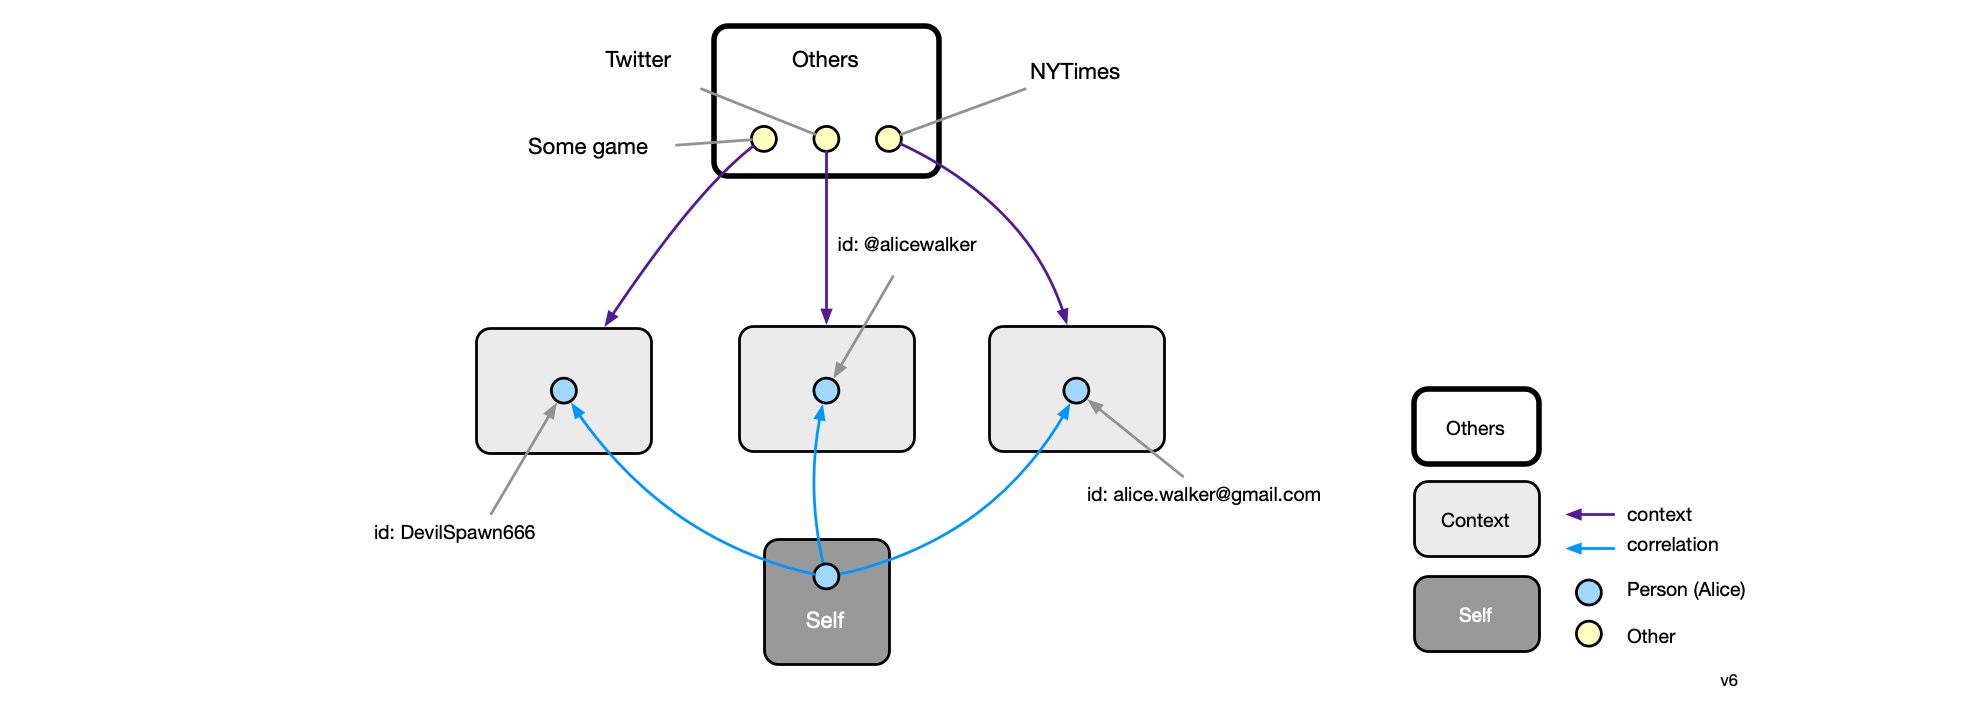
\includegraphics[width=\textwidth]{./images/example2.png}

The personal data flowing through each of the three connections represented by the purple lines above may flow from the agent, to the agent or in both directions. It may have originated on either side. It may be self asserted claims (attributes) entered by the user directly into the agent. Or it may be claims entered by the user on a website of the other party, or sensed by a local app (or sensor), or generated by the other party based on direct on-site or on-app interactions with the user.

\subsubsection{Container classes}

We describe the data model in two parts. The first part describes the data containers. The second describes the data that is held by those containers. Let us start describing the data model of the containers themselves. Here are the various data container classes: 

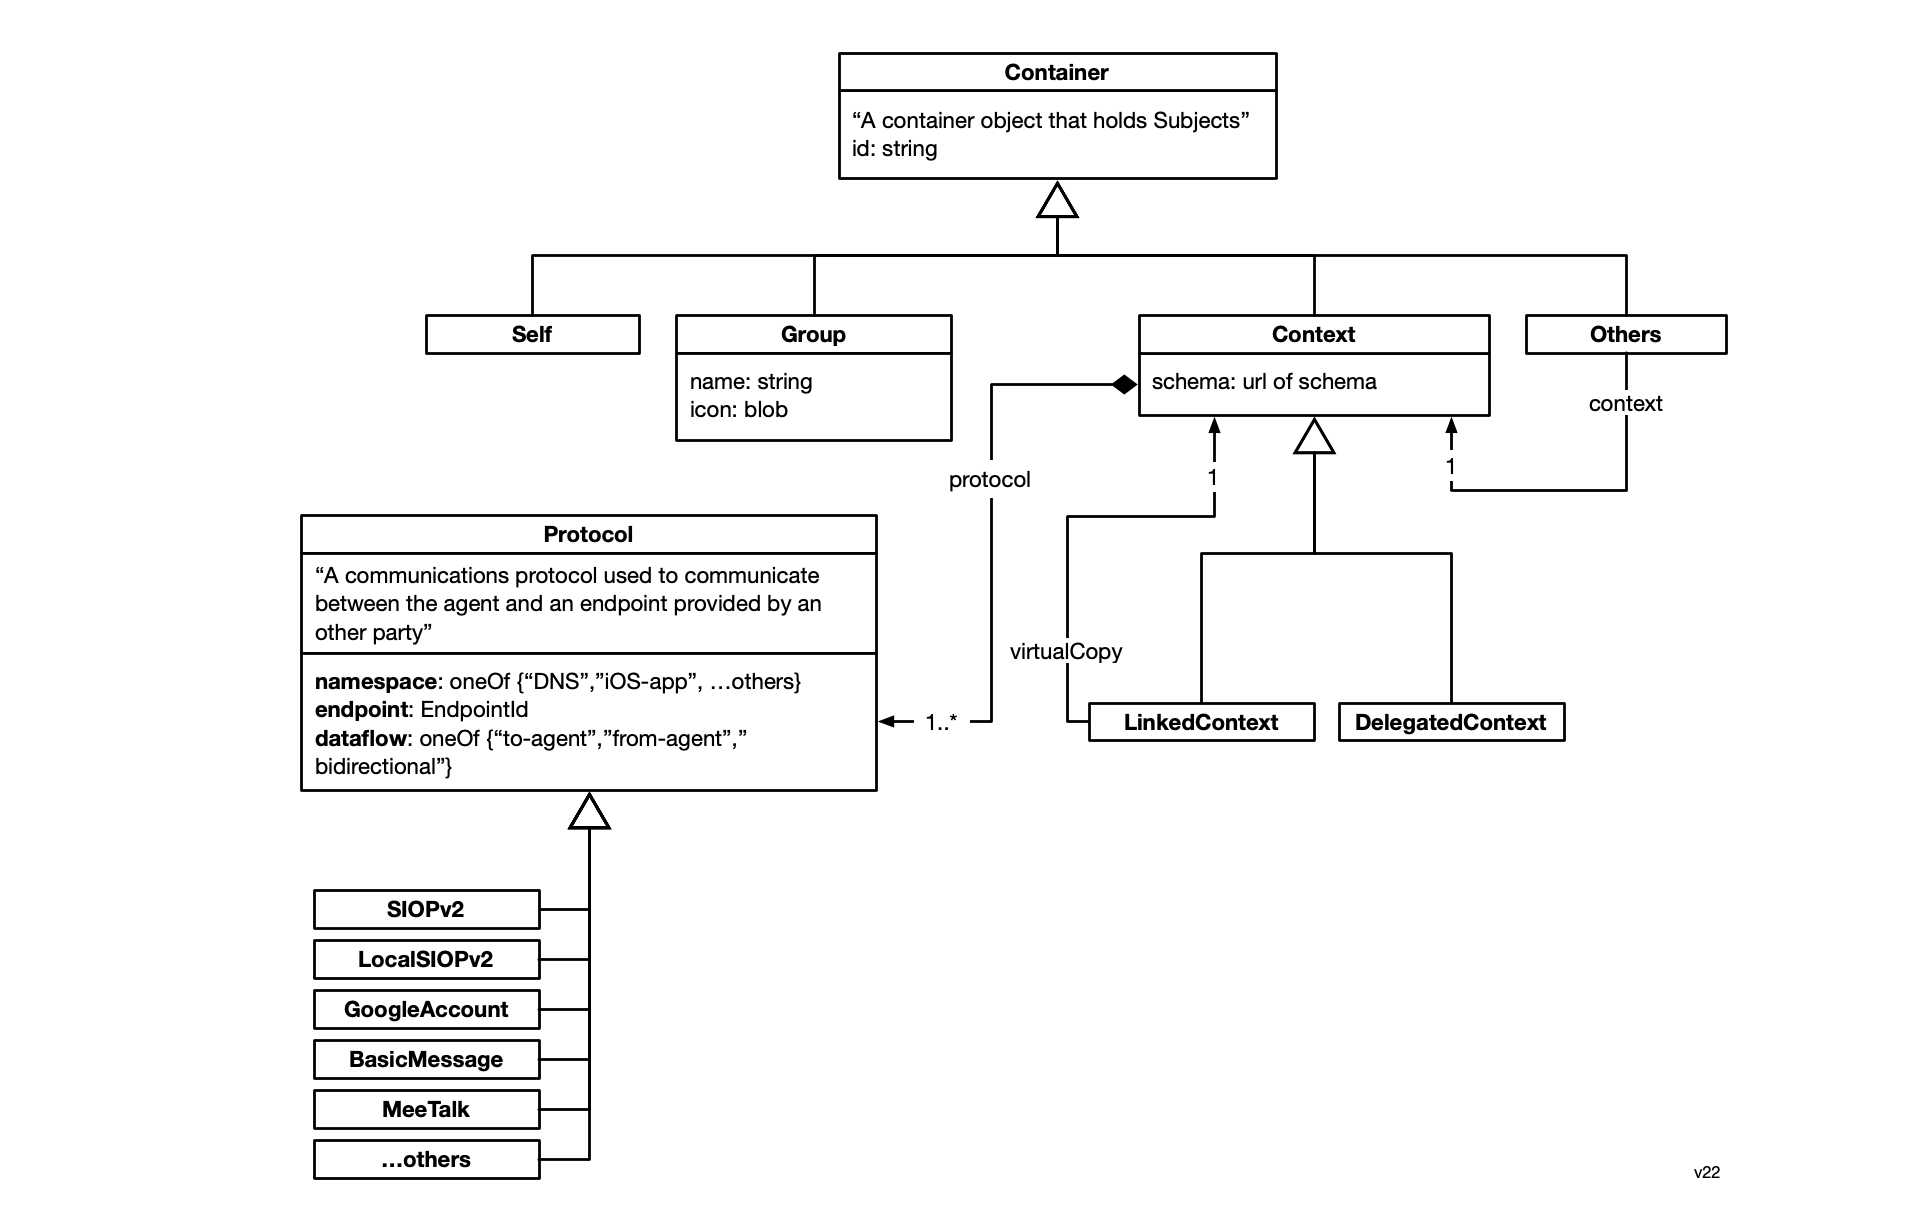
\includegraphics[width=\textwidth]{./images/container-classes.png}

\textbf{Classes}

\begin{itemize}
\item \textbf{Others} - a container holding a set of Other nodes (see Persona Classes). Each Other node represents a party with the user has a connection. These Others may be other people or legal entities. If they are legal entities, they are often called relying parties, such as a digital service provider like Twitter, Inc. Each other has the following properties:
	\begin{itemize}
	\item \textbf{Context} - a single Context that captures one aspect of the overall connection
	\end{itemize}
\item \textbf{Self} - the single Container holding a single Person node that represents the selfness of the user
\item \textbf{Group} - an intermediate level container that holds a single Person node that represents a common role or persona that the user plays. A group has these attributes:
	\begin{itemize}
	\item \textbf{name} - the name of the group 
	\item \textbf{icon} - a icon for the group
	\end{itemize}
\item \textbf{Context} - a Container holding a Person node that represents the user in a specific aspect of their relationship with some other party. We say "specific aspect" because the relationship between the user a given other, may be represented by more than one context, each representing a different aspect. 
\end{itemize}

\textbf{More about Contexts}

A context has the following attributes, that taken together uniquely identify the context:

\begin{itemize}
\item \textbf{schema} - url of the schema of the data in the context
\item \textbf{protocols[]} - array of one or more Protocol instances
\end{itemize}

The kinds of data held by a context depends on the communications protocol (using the term loosely) between the agent and the other party. As will be described next, a Protocol class within the agent represents these data conventions using a schema that is an extension of the Persona schema.

There are two subclasses of Context: \emph{LinkedContext} and \emph{DelegatedContext} that are described in their own sections below.

\textbf{Protocols}

A Protocol class represents a communication protocol used between the agent and an endpoint provided by an other party. Each protocol subclass represents a different communications protocol such as SIOPv2, GoogleAccountSync, BasicMessage (DIDComm), etc.  Protocol classes have a class method that returns the data schema used when it updates data in that context. These schemas are resolvable from a URL which is written to the *schema* attribute of the Context instance.

A Protocol is an attribute of a Context, and although a less common situation, may have more than one. Below is an example of a user Alice who has a (hypothetical) connection with Santander Bank. This connection has a single context that contains the information that Alice shares in with the bank via the OpenID Connect SIOPv2 protocol.

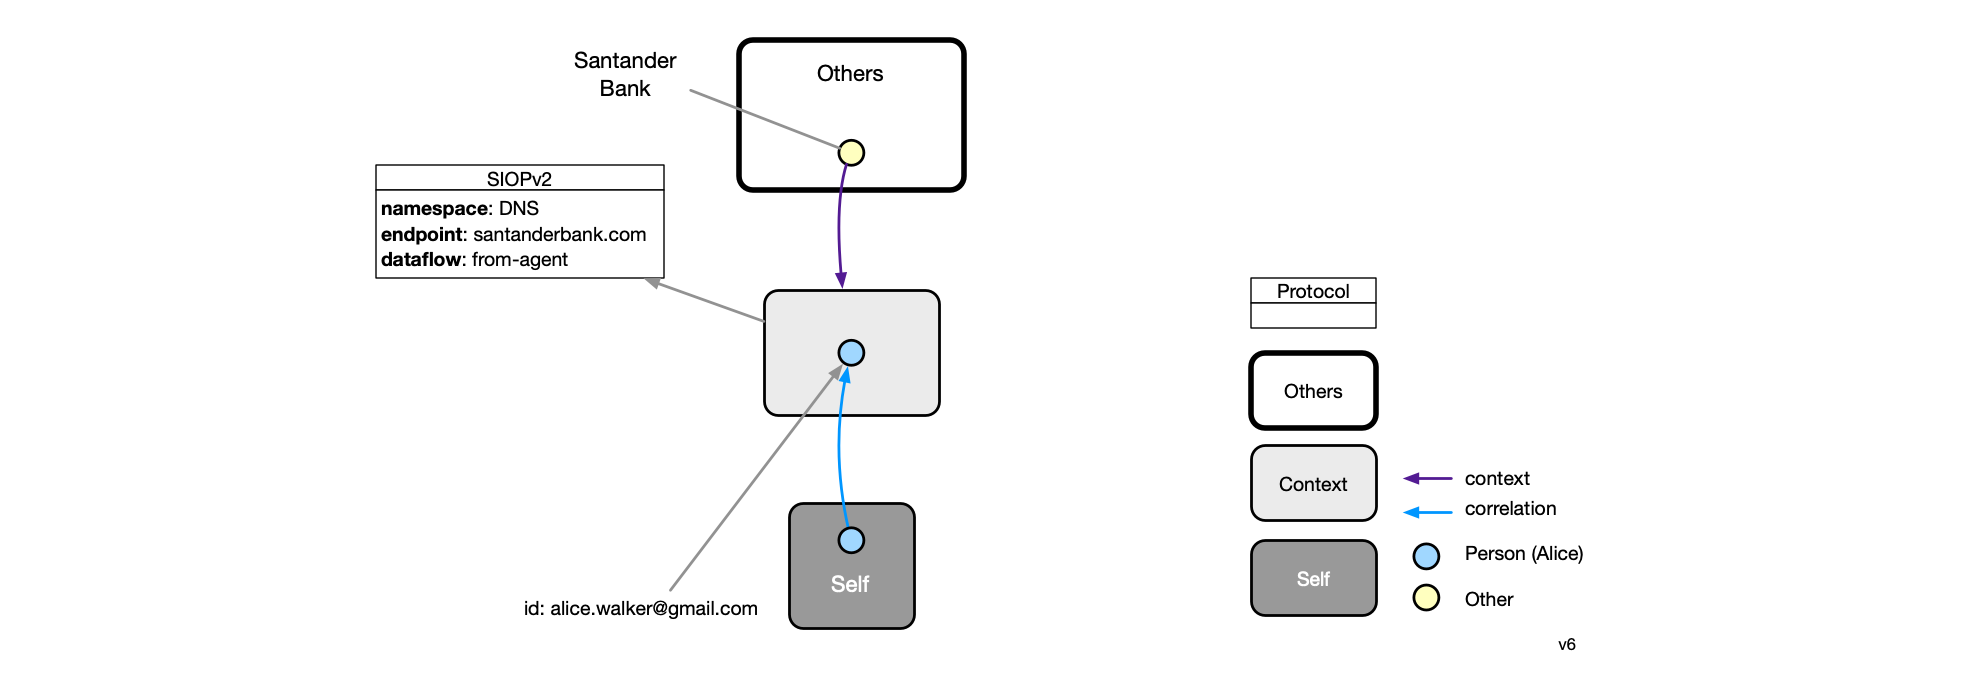
\includegraphics[width=\textwidth]{./images/context-with-protocol.png}

Each protocol instance has these attributes:

\begin{itemize}
\item \textbf{namespace} - a string that indicates the namespace used by the ``endpoint" attribute
\item \textbf{endpoint} - a string identifier that unique identifies the other party with which the user has a relationship within the above namespace attribute
\item \textbf{dataflow} - one of {to-agent, from-agent, bidirectional} - indicates the direction of data flow between the agent and the endpoint
\end{itemize}

\textbf{Multiple connections}

In the example below, we expand our story about our user, Alice. She has defined two groups. The first represents her role as a Journalist, and it contains two contexts: the context representing her relationship with Google and with Twitter. The Google context contains her Google account profile which can be updated either using her agent or via the Google website (hence the ``bidirectional" dataflow). Her Twitter context contains a snapshot of all of her Twitter account information, lists of who she follows, etc. 

The second group, entitled ``News" contains a Person linked to three context all belonging to the New York Times. The first of these three is the context that she uses, via SIOPv2 to login to the NYTimes website. The second is a context that contains data her form filler Safari extension uses. The last is a context that establishes a bidirectional connection with the NYTimes using a new (an purely hypothetical for now!) bidirectional data synchronization protocol called MeeTalk. She plays a game for which there is a context (without being within an intervening Group), and she has a direct relationship with her friend Bob using the DIDComm BasicMessage protocol.  

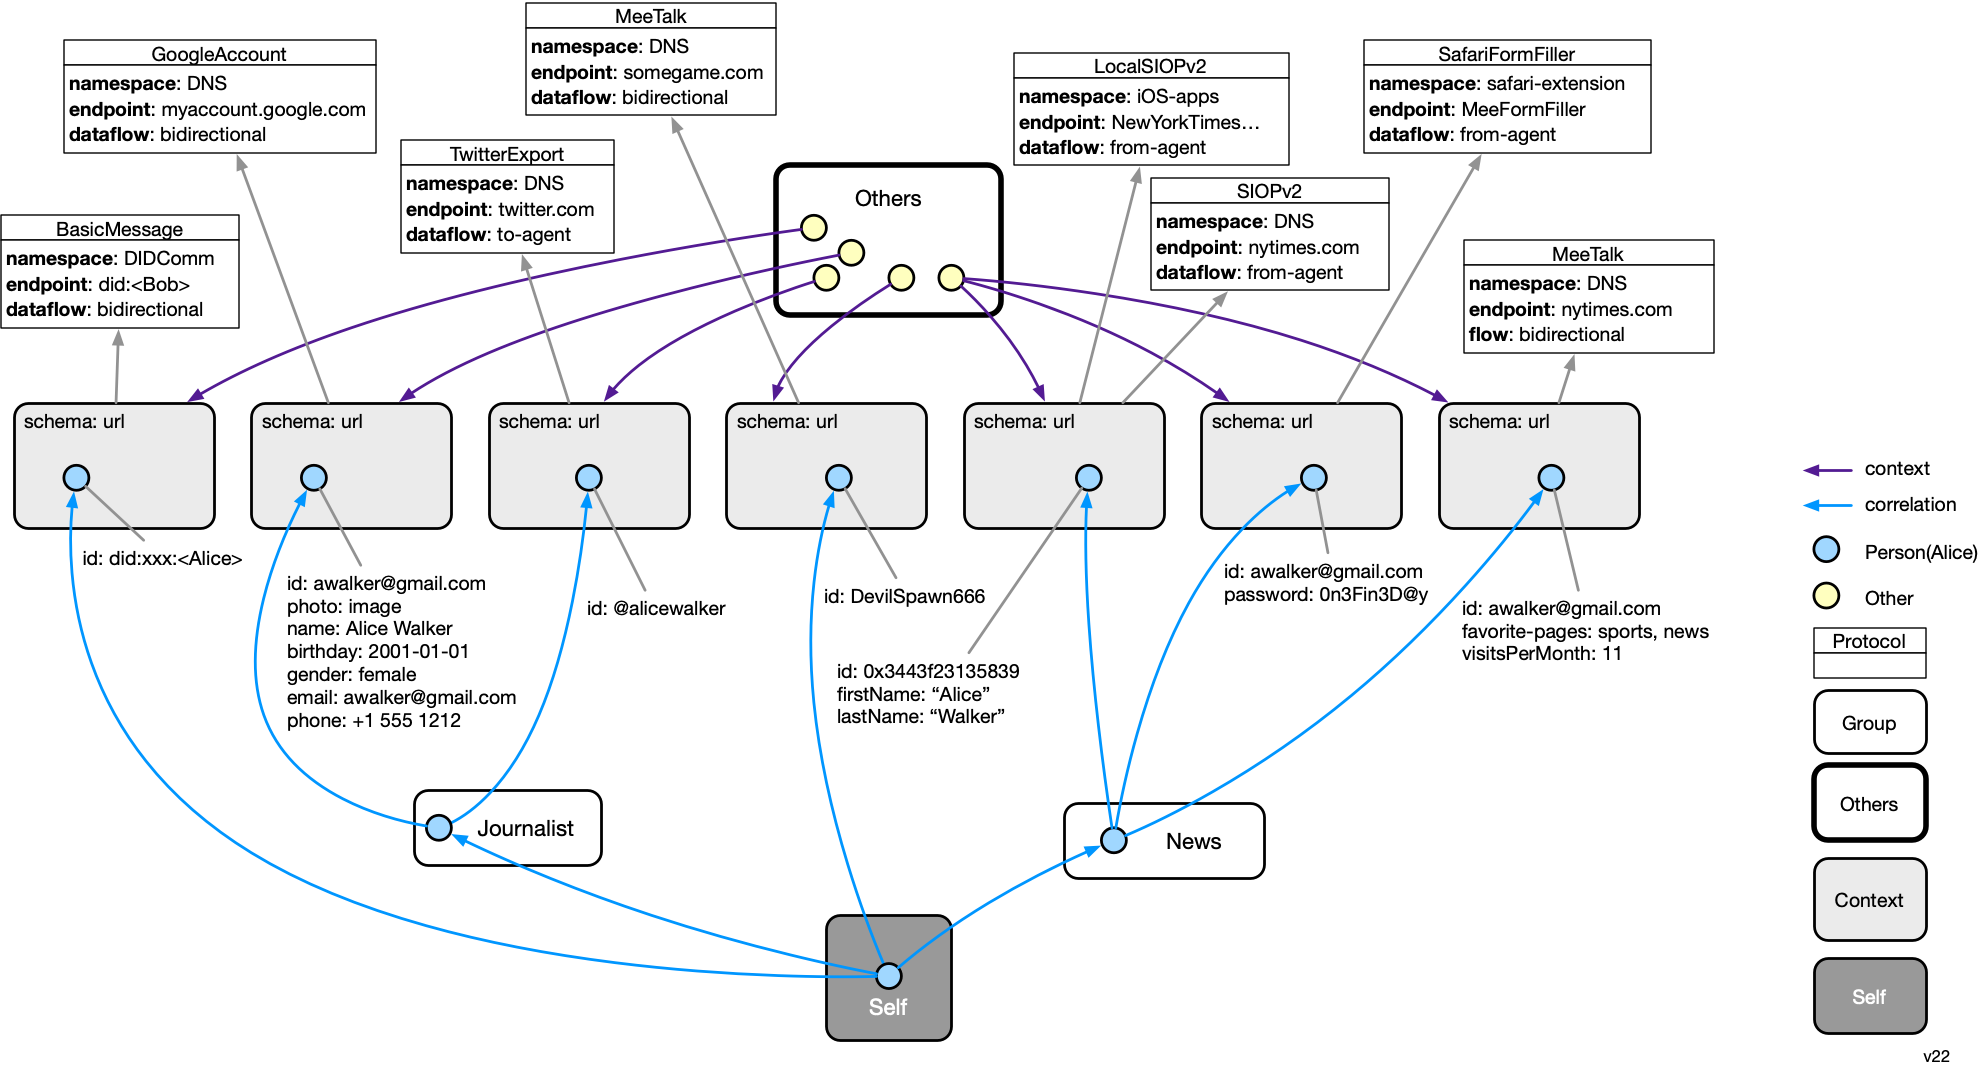
\includegraphics[width=\textwidth]{./images/multiple-connections.png}

A relationship between the identity agent and another party is called a \emph{Connection}. It is represented by one or more other contexts each of which has a protocol (and sometimes more than one). Alice is shown with five connections--one for each of the five Other nodes in her Others container. 

\textbf{Linked contexts}

Alice can convey claims made about her by one party and present them to another party. For this example we'll assume that the claims are encapsulated within a \hyperfootnote[Verifiable Credentials][https://]{w3.org/TR/vc-data-model/} document. 

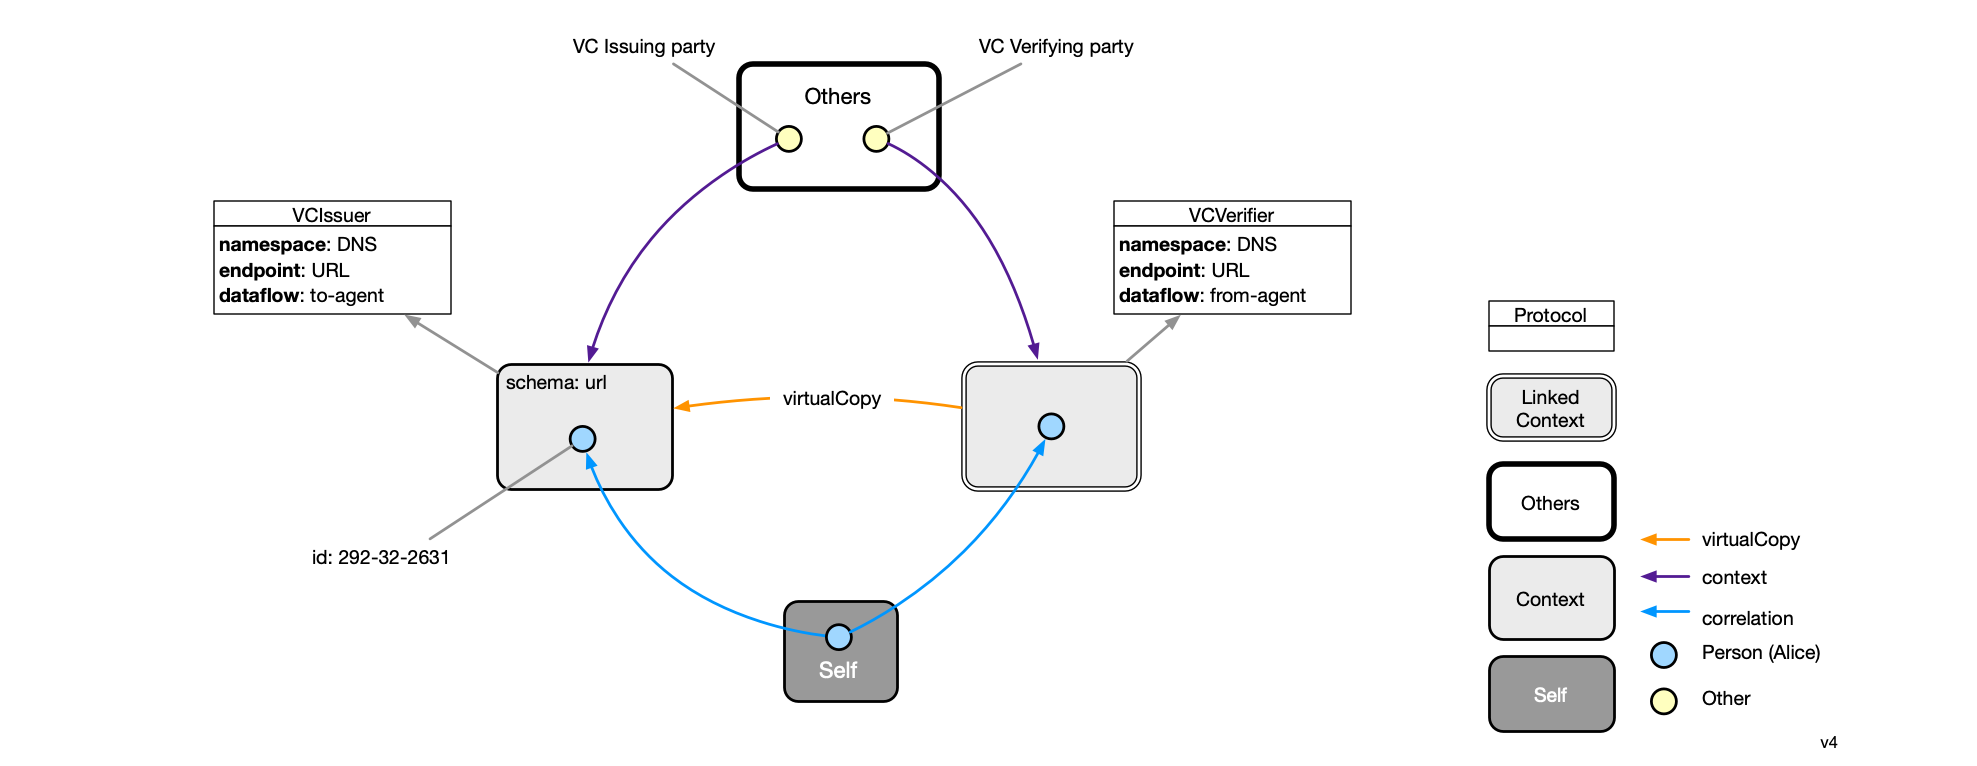
\includegraphics[width=\textwidth]{./images/linked-contexts.png}

In this example Alice, presumably having authenticated herself in her connection to a site/app of the ``VC Issuing party" is issued a VC containing claims about her which is stored in the leftmost context above. She then goes to another site/app of the ``VC Verifying party" and finds that they trust the issuing party and would accept a VC issued by them. In Alice's second connection a VC presenting protocol is used to send the VC to the verifying party. This second connection involved a special class of context, called a \emph{LinkedContext}. 

\textbf{Delegated contexts}

Alice takes care of her elderly mother, and helps her mother manage her bank account at Santander Bank. Alice's mother has an agent and has delegated access to Alice a context that contains her mother's OpenID Connect SIOP claims. 

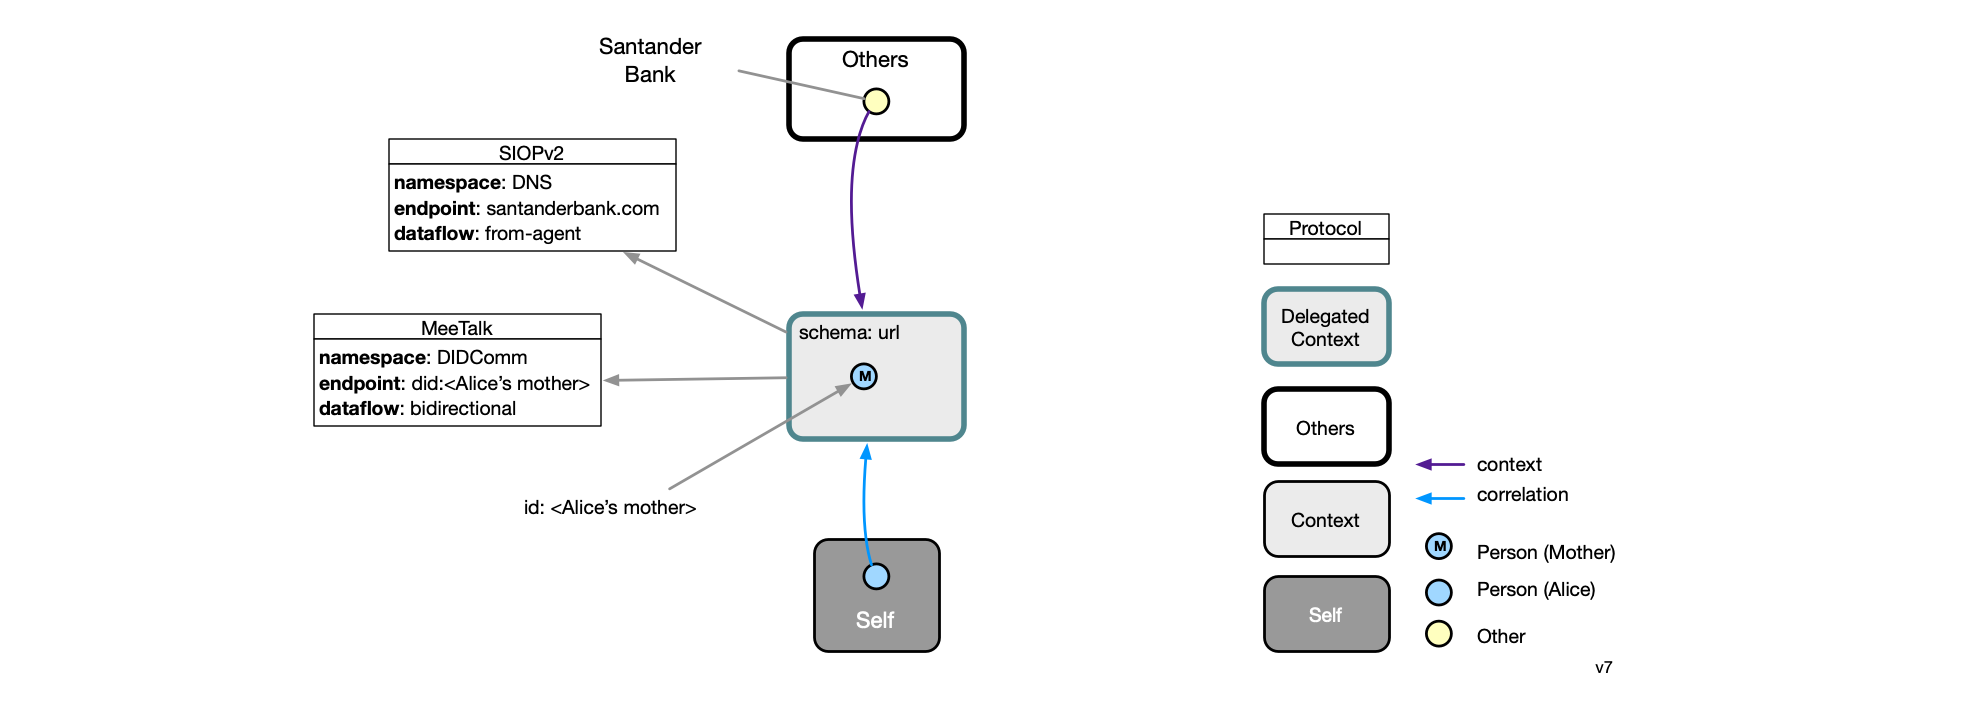
\includegraphics[width=\textwidth]{./images/delegated-contexts.png}

As shown above, Alice has a direct connection with the bank (that communicates via the SIOPv2 protocol) but the context for that connection is linked to a context managed by Alice's mother's agent. The MeeTalk data replication/sync protocol is used to ensure that Alice's DelegatedContext is always synchronized with the "original" context on her Mother's agent.

\subsubsection{Persona classes}

Group and Context containers all contain information about subjects (things) that are described according to the persona schema. In knowledge representation parlance, the Persona schema would be known as an \emph{upper ontology}.

In the Persona schema, people are be represented as instances of Person, a \emph{PersonalAccount} class is also defined. These classes are shown below. 

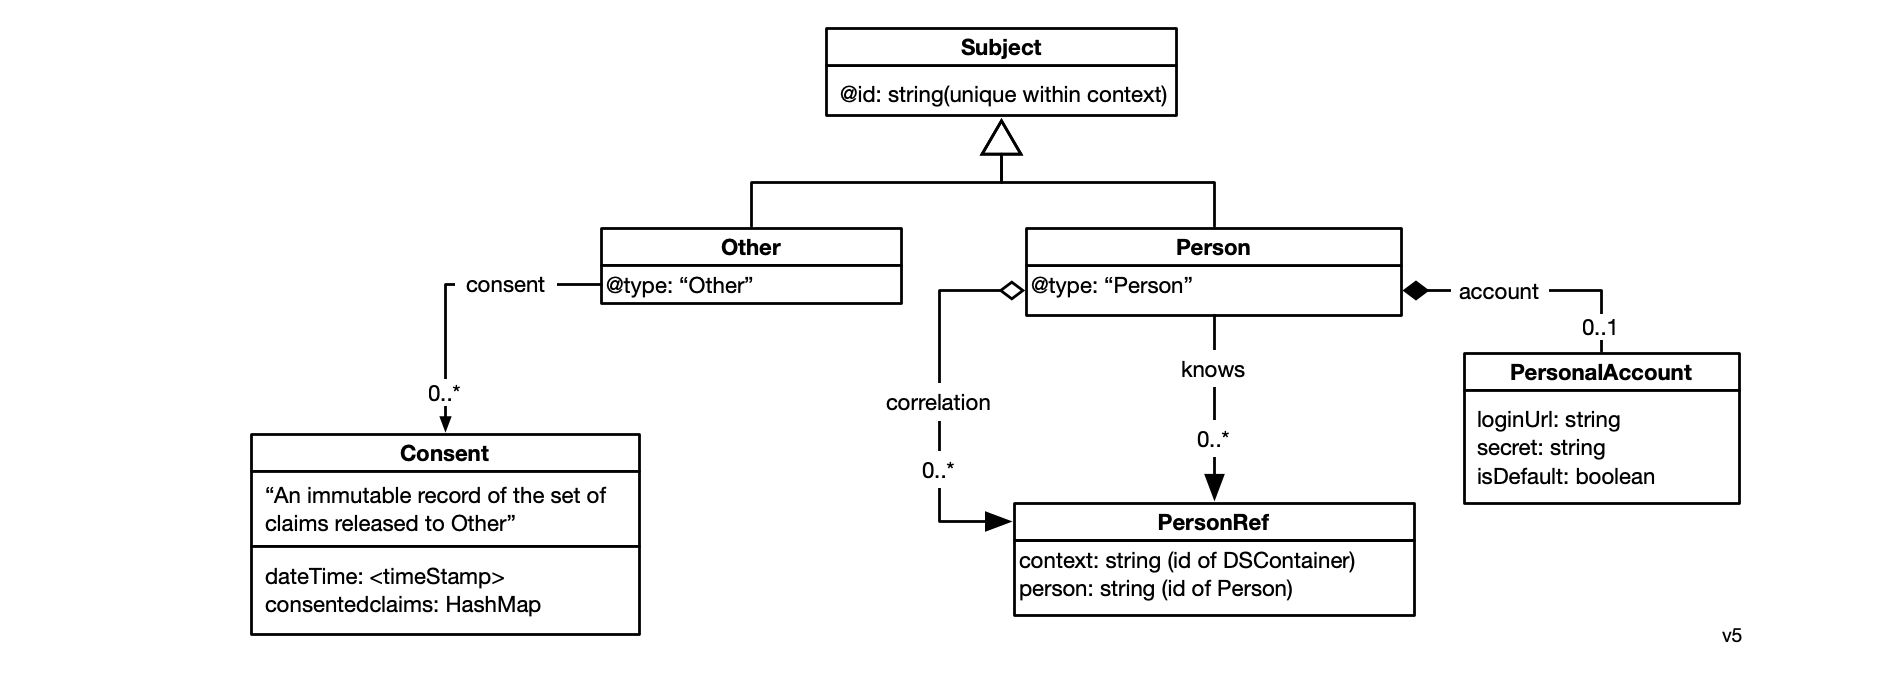
\includegraphics[width=\textwidth]{./images/persona-classes.png}

\textbf{Classes}

\begin{itemize}
\item \textbf{Subject} - kind of digital subject about which the agent stores information
\item \textbf{Person} - a natural person, a subclass of Subject. Each person has the following properties:
	\begin{itemize}
	\item \textbf{claims[]} - a set of zero or more properties. Here are a few examples: 
		\begin{itemize}
		\item givenName
		\item familyName
		\item phoneticGivenName
		\end{itemize}
	\item \textbf{account} - an optional PersonalAccount at some other party's site or app
	\item \textbf{correlation} - zero or more PersonRefs that act as a link to a target Person object representing another whoness of the link's source's person's selfness.
	\item \textbf{knows} - zero or more PersonRefs that link to a Person representing some other person (other than the user)
	\end{itemize}
\item \textbf{Other} - a Subject representing another person or a legal entity with which the user has a connection. Each Other object has:
	\begin {itemize}
	\item \textbf{consents} - zero or more Consent objects. Each Consent has:
		\begin{itemize}
		\item \textbf{dateTime} - time stamp of when the user consented to share this set of claims
		\item \textbf{claims[]}  - a set of zero or more claims (note: claim types (e.g. ``email address") not their values)
		\end{itemize}
	\end{itemize}
\end{itemize}

\textbf{Extensions}

Each protocol class will extend the Persona schema by defining Person subclasses, other new object classes and new kinds of relationships. For example the Google
\hyperfootnote[Google Account][https://]{myaccount.google.com}  API includes (optional) claims of ``name", ``gender" and ``birthday". The protocol that supports the myaccount API would define these claim types in its schema, and insert a link to this schema in its corresponding context's \emph{schema} attribute.

\subsubsection{Datatypes}

This section is largely incomplete, but will eventually describe lower level classes that we call datatypes that are used by the higher level classes mentioned above.

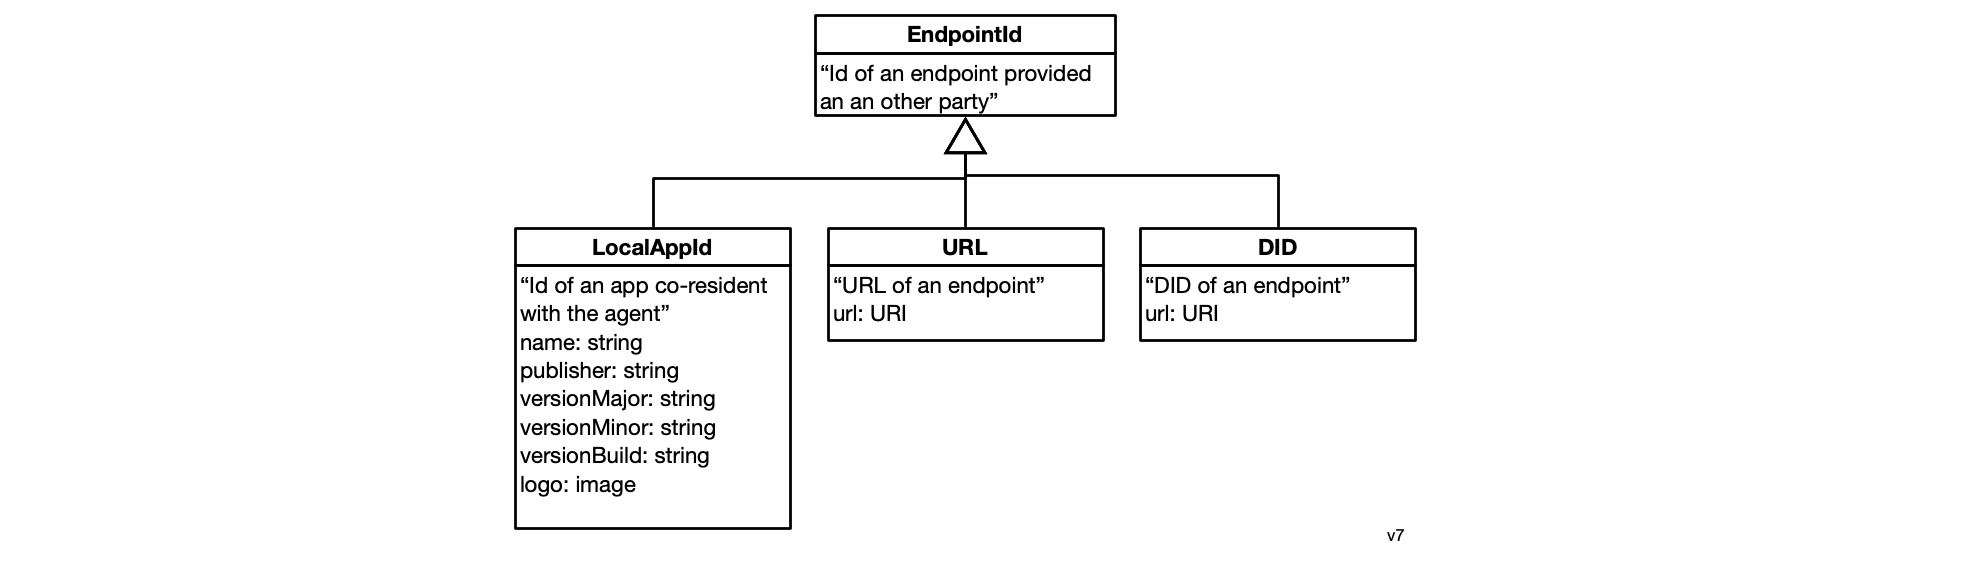
\includegraphics[width=\textwidth]{./images/datatypes.png}

\begin{itemize}
\item \textbf{EndpointId} -  an identifier of an endpoint (e.g. webservice or a local app) supported by an other party.
\item \textbf{LocalAppId} - A specific kind of EndpointId. Uniquely identifies a service provider's mobile app. 
\item \textbf{Secret Recovery Phrase} - a 12-word textual phrase that the user creates. It is used to generate cryptographic keys that in turn are used to encrypt the user’s personal data whether it is stored locally on their device or in a backup location. It can be used to generate keys to digitally sign transactions (e.g., for crypto currency transactions). It should never be shared with anyone or any service provider. If the user loses this phrase, they lose the ability to decrypt their data. 
\end{itemize}

\section{Agents and apps} % SECTION 

We now consider agent interactions with apps and websites. 

\subsection{Interactions}

In the diagram below Alice's agent in the \emph{Agent} layer is interacting with apps in one of two \emph{Application Layers}. The top application layer contains two apps running on a remote system. The first is \emph{Bob's Agent} which appears to Alice as an app (just as, by symmetry, Alice's agent appears as an app to Bob's agent). The second is a website labeled \emph{Provider's Website}. The lower application layer contains \emph{local apps} that run on the same device where Alice's device agent is also running. The digram shows a local app labelled \emph{Provider's Local App}.

The first step setting up a connection with a provider's app for the app to authenticate the user's agent. We app implements the \hyperfootnote[OpenID SIOPv2][https://]{openid.net/specs/openid-connect-self-issued-v2-1\_0.html} for this purpose. After authentication, a private data sharing connection can be established.

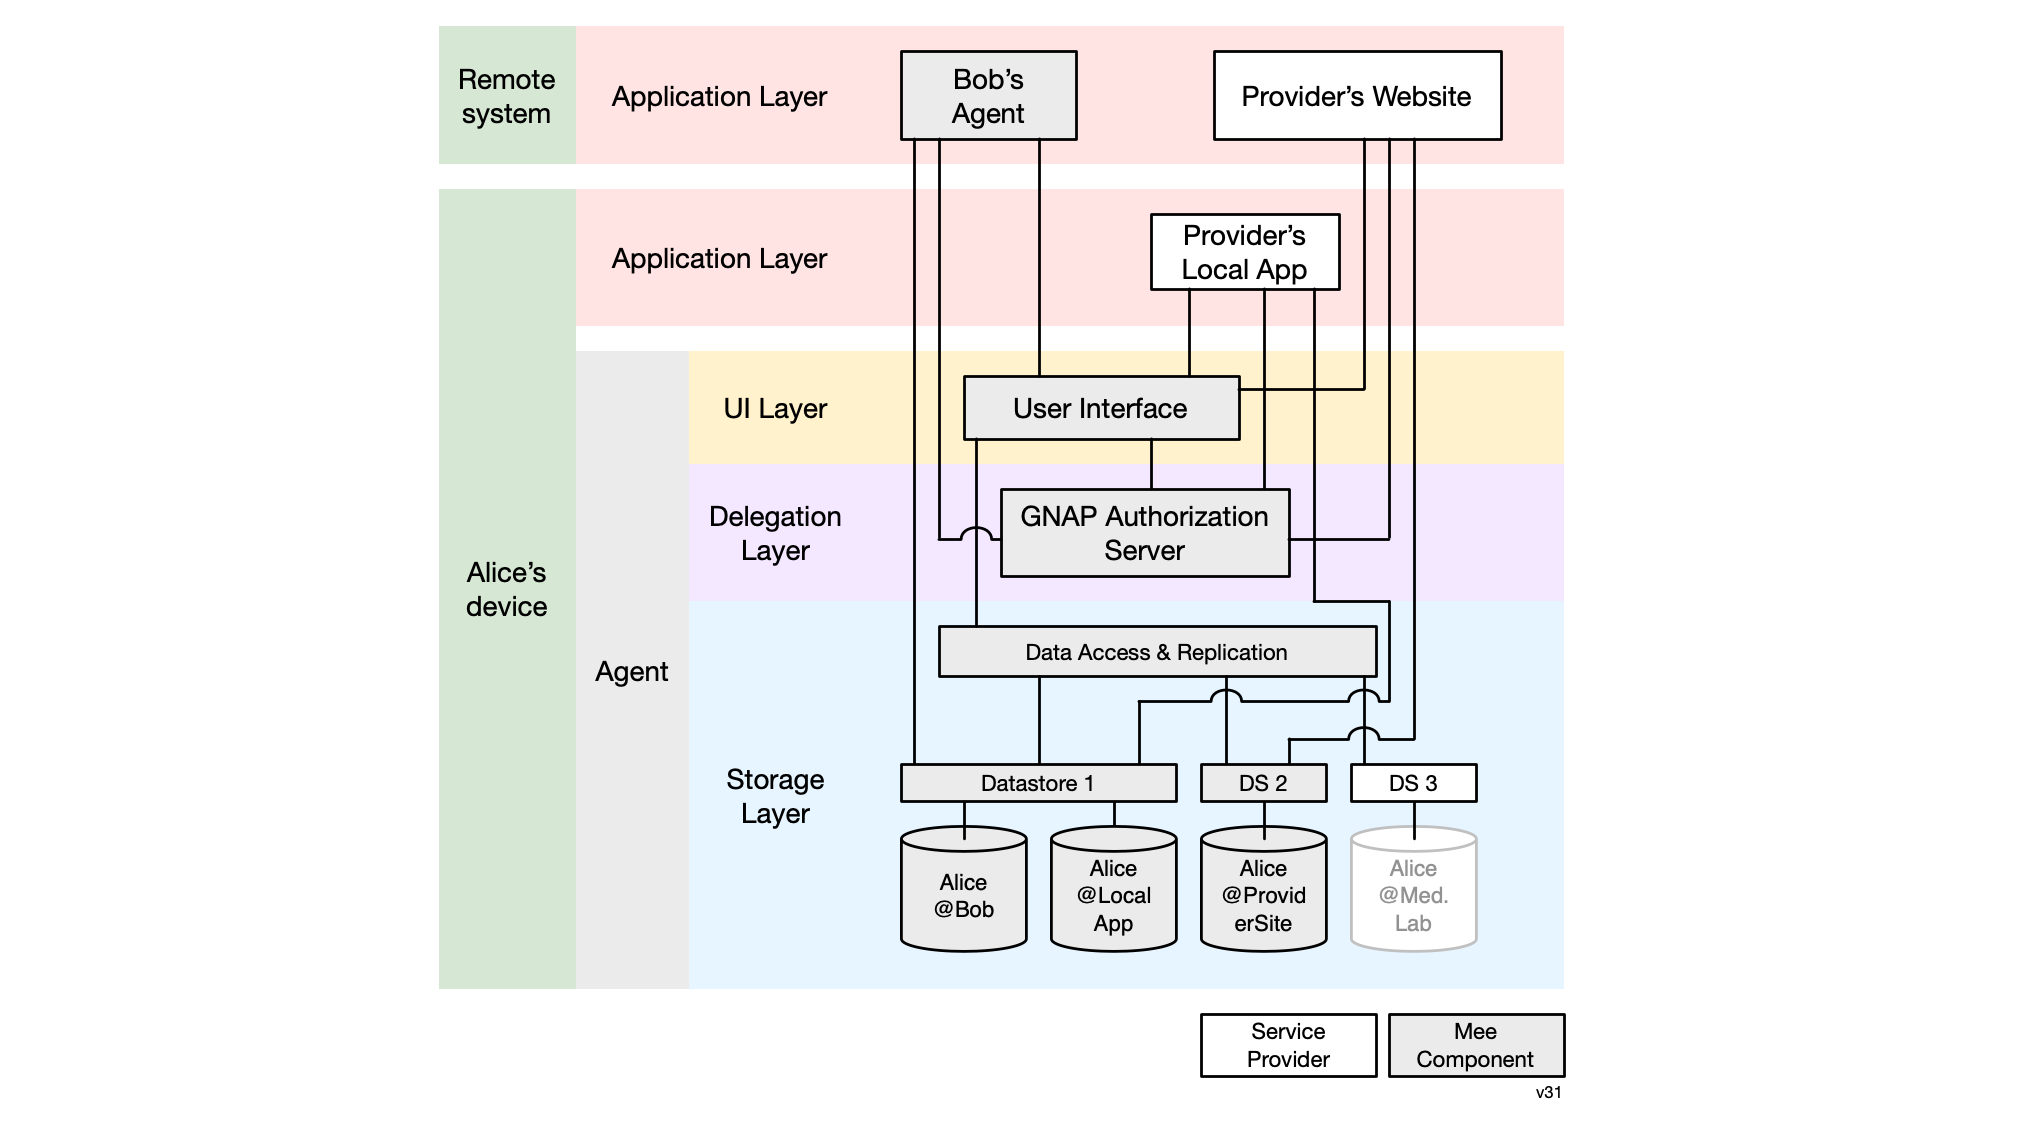
\includegraphics[width=\textwidth]{./images/applications.png}

\subsection{Private data sharing}

Data held and/or managed by the user's agent is clearly under the user's control. The challenge is that data that the user has shared with another party \emph{also} needs to be under their control. Since no technical means exist to control a user's data held by another party, we must rely on law. Current privacy laws and regulations are intended to provide this control, but place such burdens on the user to effectuate their control that this control hardly exists. The solution we proposed is to combine both legal (license agreement) and technical means (identity agents). 

The legal mechanism we propose is a \hyperfootnote[Human Information License (HIL)][https://]{docs.google.com/document/d/13aGk5adoncMxxfl5637NfqP6fl6q\_op\_1CF50UrJNjg}. The (HIL) contract between two parties. The first is the digital service provider legal entity behind a given app. The second is a legal entity, The Mee Foundation, a nonprofit that represents agent users. The HIL imposes a number of obligations of the provider. Among them is the provider's requirement to respect the user's \emph{data rights} to access, correction (editing), and deletion of the information collected and held by them. The user may have shared information manually (e.g. by filling in a form, or other kinds of interactions) or online from their agent. The HIL requires the provider to implement \emph{data rights} APIs/protocols that an agent can use to remotely control this collected data. In this way we tie the legal (HIL) and technical means (agents and APIs) together.


\section{Contributors}
Contributors to this document include Kiril Khalitov, Sergey Kucherenko, Maria Vasuytenko, and Alexander Yuhimenko.

\bibliography{library}
\bibliographystyle{plainurl}


\end{document}  